%\usepackage{here}
%\usepackage[dvipdfmx]{graphicx}
%\usepackage{amsmath,amssymb}
%\usepackage{array,booktabs} %表のためのarray環境

%\begin{document}
\section{NaIで取得したデータの解析と結果・考察}
以下では主に測定した信号から欲しい情報を取り出すための解析に関する部分と,得られた情報から実際の測定した量を解析する部分にわけて,解析の詳細を述べる.
特に前半の信号解析ではパイルアップ信号を取り除く処理を行い,情報を取り出す解析を行った.
後半では寿命と$g$ 因子の測定をフィッティングを用いて行った.
また,ミッシェルパラメータの測定では時間情報に基づいたスピンの情報とエネルギーの相関を含めた解析を行った.
その際,各NaIで得られたエネルギー情報に対し測定器の電磁シャワーの応答に基づくフィッティングを行った.

\subsection{信号解析}
NaI 検出器で測定した波形解析の手法について述べる.
測定波形の中で典型的なものを\figref{hatano_fig:rawdata} に示す.
波形解析ではここからフィンガーカウンター(チャンネル1 )が鳴っているという条件を課したときにNaI で測定したエネルギーと信号の時刻という2 つの情報を抽出した.
この際に信号のノイズとNaI と波形の重なり(以下,パイルアップとよぶ)の2 つが解析時の注意点となった.
前者は信号が鳴ったという判定をするためのピーク検出をする際に問題となる.
具体的には,本来1 つの$e^+$ からの信号であるのにノイズの影響で複数のピークとして認識してしまう.
そのため,今回の解析ではノイズ除去の処理を最初に行った.
その後ピーク検出を行った後に時間情報とエネルギー情報を取り出す.
この際にパイルアップの処理をしないまま適当な領域で積分を行いエネルギーを求めると,別の$e^+$ からの信号でエネルギーが大きく見積もられてしまう.
このため,今回の解析では波形データのサンプリングを行い,それに基づきパイルアップしてない部分の波形からパイルアップしている部分に外挿し,その分の補正を行った.
以下具体的な処理について述べる.

\begin{figure}[hbt]
\centering
\includegraphics[width=0.6\textwidth]{figure/hatano/rawdata_modify1.eps}
\caption{NaI 検出器の測定信号.チャンネル1 はフィンガーカウンターの測定波形,チャンネル3 〜チャンネル7 はNaI の測定波形.NaIの測定波形では波形の重なりが見られる.}
\label{hatano_fig:rawdata}
\end{figure}

\subsubsection{ノイズ除去}
ピーク検出の際に問題となる高周波のノイズを除去することについて考える.
高周波成分によるピークと誤認識するような大きな変動がなくなればいいので,簡単に実装ができかつ高速な処理ができるという観点で単純移動平均をとるということを行った.
具体的には各サンプリング点で前後4 サンプリング,計9 サンプリングの平均をとった.
実際にノイズ除去を行った前後の信号の差異は\figref{hatano_fig:smoothdata}(\figref{hatano_fig:smoothdata} と同じデータの一部)のようになった.
チャンネル6 の左側の信号はノイズによって2 つのピークのように見かけ上分裂していたのが改善しているのが分かる.

\begin{figure}[hbt]
\centering
\includegraphics[width=0.6\textwidth]{figure/hatano/smoothdata_modify1.eps}
\caption{ノイズ除去された測定信号.薄い色で示したのが元の信号,濃い色で示したのがノイズ除去を行った信号.チャンネル6 の信号はノイズによって2 つのピークのように見かけ上分裂していたのが改善している.}
\label{hatano_fig:smoothdata}
\end{figure}

\subsubsection{ピーク検出}
以上のノイズ除去を行った信号を元にピーク検出を行うことを考える.
基本的にはthresholdを適切に設定しそれを超えたところからピークが始まったと考えることにする.
ただし,この方法ではパイルアップしている際には過剰に信号を検出してしまう可能性がある.
すなわち,別の信号と重なってそれがオフセットになりthreshold が下がっているのと同じ状態になり,低エネルギーの信号を拾いやすくなる.
そのため,threshold のbaseline となる値を信号が来る前の最小値とすることにした.その手法の模式図を\figref{hatano_fig:threshold}に示す.

\begin{figure}[hbt]
\centering
\includegraphics[width=0.6\textwidth]{figure/hatano/threshold.eps}
\caption{ピーク検出の模式図.青線と緑線で示したのが入射した粒子毎に対応する信号.赤線で示したのが青線と緑線の信号を合わせた測定信号.薄い青で示した矢印がthreshold の高さである.緑線に対応する信号はthreshold 以下であり検出されない.}
\label{hatano_fig:threshold}
\end{figure}

このような工夫をすることで,パイルアップしている際はbaseline が高くなるため,パイルアップによるオフセットの影響をある程度キャンセルすることができる.
そのようにしてピーク検出を行った際の信号が\figref{hatano_fig:peakdata} である.

\begin{figure}[hbt]
\centering
\includegraphics[width=0.6\textwidth]{figure/hatano/peakdata_modify1.eps}
\caption{ピークとして検出された信号.それぞれ色が濃くなっている部分がピークまでの立ち上がりとして判定されている領域で,点で示されているのがピーク(最大値)である.}
\label{hatano_fig:peakdata}
\end{figure}

\subsubsection{波形データの抽出}
パイルアップに対処するために全イベントからパイルアップしていない時の波形データを抽出しそれにより外挿を行うことを考える.
NaIは減衰時間が長く主にその部分でパイルアップが起きていると考えた.
すなわち,ピークの部分は全て検出できているとし立ち下がる部分によるパイルアップのみに対処した.
具体的には波形データのサンプルから減衰時間を測定し,それを元にピークから立ち下がり部分に$\exp(-t/\tau)$ ($\tau$: 減衰時間)の関数を仮定して外挿をするというアプローチをとった.
まず,ピーク検出された信号のうちパイルアップしていない信号の減衰部分に対して指数関数でフィッティングを行った.
パイルアップしていない信号は,次のピーク信号がくるまで400~ns 以上の間隔があるものと定義した.
また減衰部分の領域はピーク部分の影響やバックグラウンド部分の影響を減らすため,ピークから80~ns 後から次の信号が来るまでの最後の10~\% を外した領域とした.
これに対してフィッティングを行いその$\chi^2$ のConfidence Level (CL) が50~\% を切るものは解析には使用しなかった.
実際のフィッティングを行った時の様子が\figref{hatano_fig:decayfit} である.濃い色で示されているのがフィッティングした関数であり,赤の線で示したのはCL が50~\% 以下であったため用いなかった信号である.

\begin{figure}[hbt]
\centering
\includegraphics[width=0.6\textwidth]{figure/hatano/decayfit_modify1.eps}
\caption{波形データに対するフィッティング.濃い色で示されているのがフィッティングした関数であり,赤の線で示したのはCL が50~\% 以下であったため用いなかった信号である.}
\label{hatano_fig:decayfit}
\end{figure}

これを全ての測定データに行い,減衰時間の分布を求めた結果が\figref{hatano_fig:decaytime} である.
チャンネル7 のヒストグラムは2 峰になっているが,これは異なる減衰特性の2 つのNaI の信号をアナログ的に加算したためと考えられる.
他のチャンネルのデータのピーク値もある程度のばらつきがある事が確認される.
また外挿の際にはピークからそれがアナログ的に加算したNaI のどちらからの信号であるかを識別する事はできないため,これらを選別することを考えず各チャンネル毎に減衰時間を単純に平均し,それを減衰時間とした.

\begin{figure}[hbt]
\centering
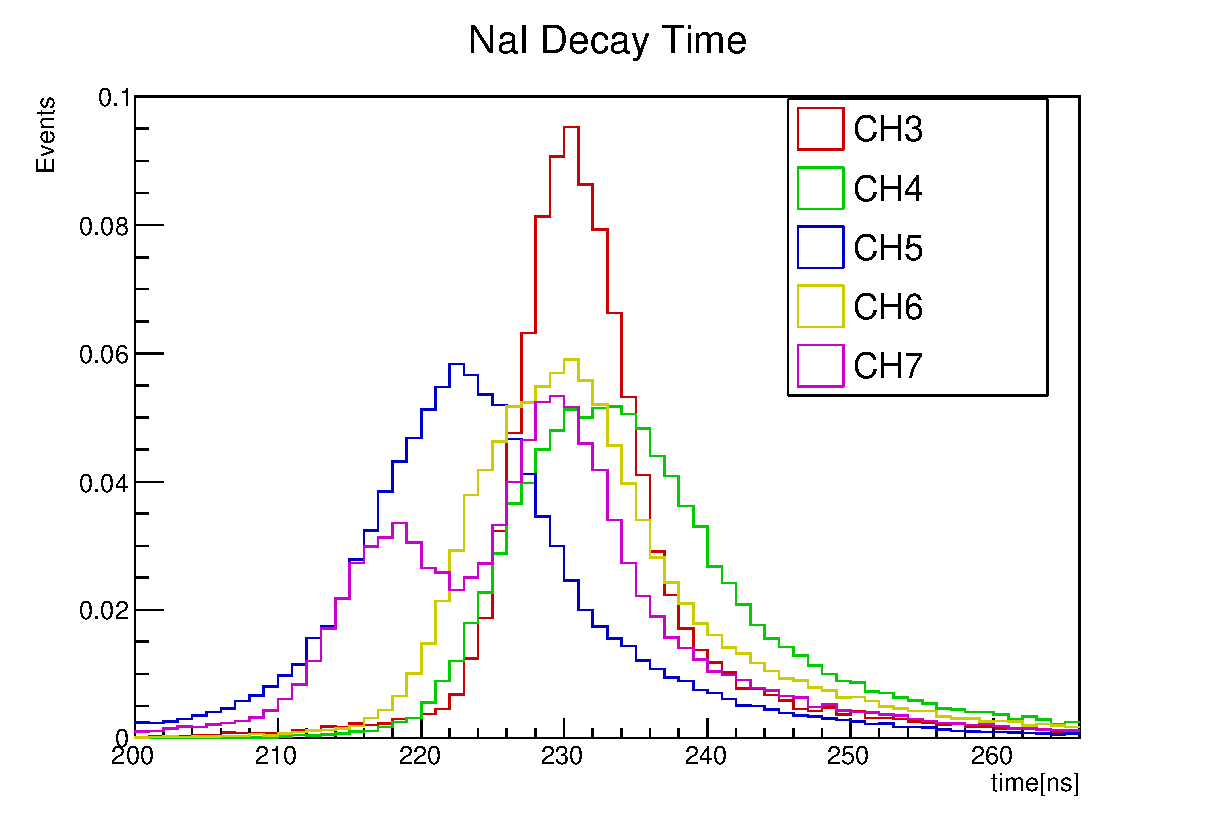
\includegraphics[width=0.6\textwidth]{figure/hatano/decaytime.eps}
\caption{NaI の減衰時間の測定.チャンネル7が2峰あるのは異なる減衰特性の2つのNaIの信号をアナログ的に加算したためと考えられる.}
\label{hatano_fig:decaytime}
\end{figure}

その結果が\tabref{hatano_tab:decaytime}である.

\begin{table}[hbt]
\centering
\caption{各チャンネルにおける減衰時間}
\begin{tabular}{cc}\\ \toprule
チャンネル番号 & 減衰時間~[ns]\\ \midrule
3 & 232.6 \\
4 & 236.7 \\
5 & 224.2 \\
6 & 233.4 \\
7 & 228.6 \\ \bottomrule
\end{tabular}
\label{hatano_tab:decaytime}
\end{table}

\subsubsection{波形データの外挿}
波形データの外挿は次のように行った.
ピークが終わった後の減衰中に次のピークが見つかった場合は,減衰時間中の最小値から前5サンプリング分のデータを基準に求めた減衰時間(\tabref{hatano_tab:decaytime}) の指数関数を外挿した.
実際に外挿を行った時の信号の様子が\figref{hatano_fig:analysis} であり,濃い色の線で示しているのが外挿した波形データである.

\begin{figure}[hbt]
\centering
\includegraphics[width=0.6\textwidth]{figure/hatano/analysis_modify1.eps}
\caption{波形の外挿の様子.濃い色の線で示しているのが外挿された波形データ.点で示しているのが各信号の時間と定義されたところ.}
\label{hatano_fig:analysis}
\end{figure}

\subsubsection{解析データの抽出}
以上で各チャンネルごとに信号から時刻とエネルギーの情報を抽出する準備ができたので,これを元にピークの50~\%の値を超えたところを信号の時刻として,前のピークから外挿された分を差し引き,自らの外挿分を加えた積分値をエネルギーとした.

必要なデータは標的から飛んできた陽電子が手前のフィンガーカウンターを通った事象のものだけであるので,フィンガーカウンターの信号と同時に鳴ったとみなせるNaI 信号を選ぶことを考える.
フィンガーカウンターと各NaI信号の時間差をとると\figref{hatano_fig:coincidence}のようになった.
この分布より,フィンガーカウンターが鳴った時を基準にその後20~nsの間に鳴ったNaI 信号をフィンガーカウンターと同時に鳴ったものと定義した.

\begin{figure}[hbt]
\centering
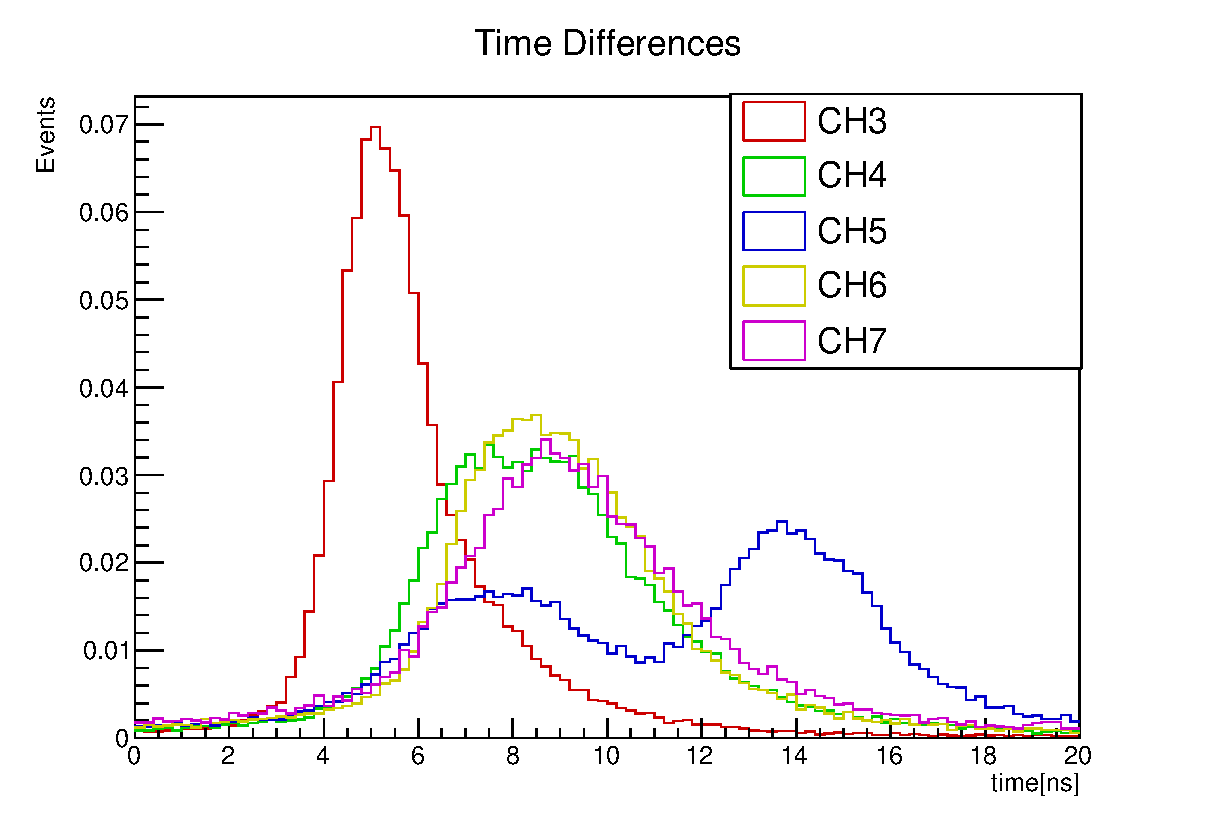
\includegraphics[width=0.6\textwidth]{figure/hatano/coincidence.eps}
\caption{フィンガーカウンターと各NaI の時間差}
\label{hatano_fig:coincidence}
\end{figure}

%%%%%%%%ここから三野の続き%%%%%%

\subsection{NaI を用いた寿命と$g$ 因子の解析}
\subsubsection{使用データ}
寿命測定用に磁場なしで測定を行ったRUN15,$g$ 因子測定用に磁場ありで走ったRUN18, RUN19 のデータを用いて解析を行った.
RUN15における波形記録のサンプル数は250MHzで1030点,ビーム信号が到達してから4120~nsの波形を記録した.
RUN18 とRUN19 のサンプル数は2050 点で8200~ns の時間までの波形を記録した.
解析に用いたデータを表\ref{tab:RUN_info} にまとめる.

\begin{table}[H]%RUN Information
\caption{用いたRUN の情報}
\centering
\begin{tabular}{cccc}\toprule
{} & $B~[\mathrm{G}]$ & Time~[min] & Event数\\ \midrule
RUN15 & --- & 47 & 71532 \\
RUN18 & 56.06 & 75 & 113584 \\
RUN19 & 53.97 & 297 & 446578 \\ \bottomrule
\end{tabular}
\label{tab:RUN_info}
\end{table}

図\ref{fig:no_mag}-\ref{fig:with_mag_RUN19} は磁場なしと磁場ありで中心のNaI とフィンガーカウンターでコインシデンスを取った場合の時間分布である.
% コインシデンスという表現でいいか?
\begin{figure}[H]
\centering
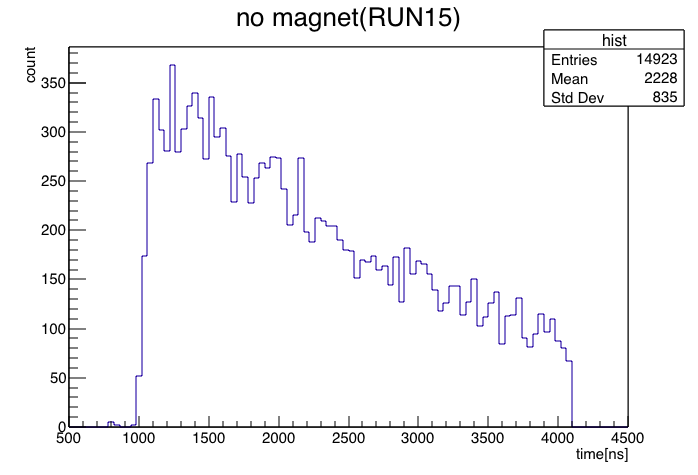
\includegraphics[width  = 0.5\textwidth]{figure/mino/no_mag.eps}
\caption{磁場がないときの時間分布 (RUN15)}
\label{fig:no_mag}
\begin{minipage}{0.45\hsize}
\centering
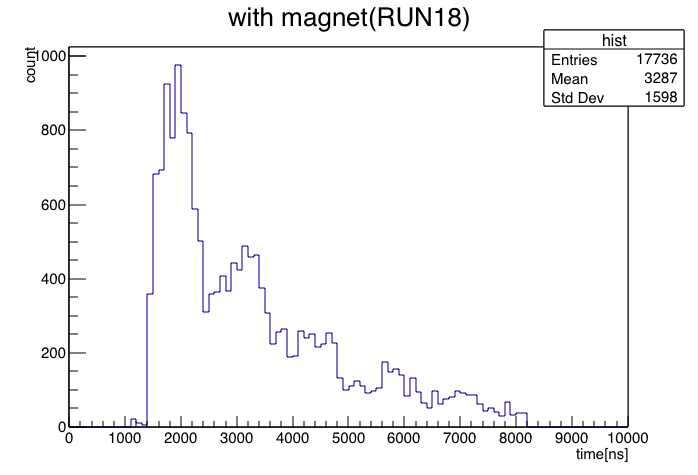
\includegraphics[width  = 1.0\textwidth]{figure/mino/with_mag_RUN18.eps}
\caption{磁場があるときの時間分布 (RUN18)}
\end{minipage}
\begin{minipage}{0.45\hsize}
\centering
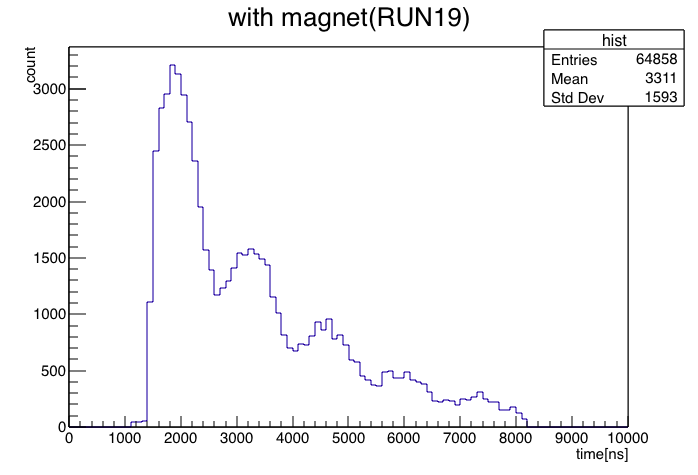
\includegraphics[width  = 1.0\textwidth]{figure/mino/with_mag_RUN19.eps}
\caption{磁場があるときの時間分布 (RUN19)}
\label{fig:with_mag_RUN19}
\end{minipage}
\end{figure}

%--------- peak ratio -----------------------------------------------------------

\subsubsection{時間分解能}
ピークに対する一定の高さの比 (50~\%) を超えたところを信号の時刻として用いて,寿命と$g$ 因子を求めた.
図\ref{fig:Original} に,縦軸がNaI とフィンガーカウンターの時間差,横軸が中心のNaI で落としたエネルギーの分布を示す.
中心のNaI とフィンガーカウンターでコインシデンスを取った時のイベントのこの図から,エネルギーに対して時間差がほとんど一定で信号の時刻の補正は必要ないことを確認した.

\begin{figure}[H]%TQ compensation check
\centering
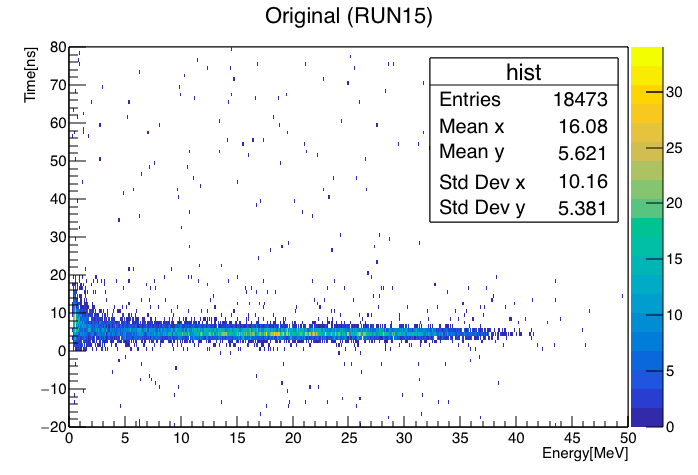
\includegraphics[width  = 0.5\textwidth]{figure/mino/Original.eps}
\caption{中心のNaI とフィンガーカウンターの時間差}
\label{fig:Original}
\end{figure}

ただし,低エネルギーでは波形信号が小さい影響で高エネルギー側と比べて時間分解能が悪いため,5~MeV より高いエネルギーの信号を用いて解析を行った.図~\ref{fig:NaI_peak_gaus_fitting} は0-4~MeVの低エネルギーのイベントを1~MeV 毎に区切って時刻をガウシアンでフィッティングしたものである.
また,図~\ref{fig:NaI_peak_time_resolution} はフィッティングで得られたガウシアンの$\sigma$ を,エネルギーの関数としてプロットしたもので,低エネルギーは時間分解能が悪いことが確認できる.

\begin{figure}[H]%time resolution
\begin{minipage}{0.5\hsize}
\centering
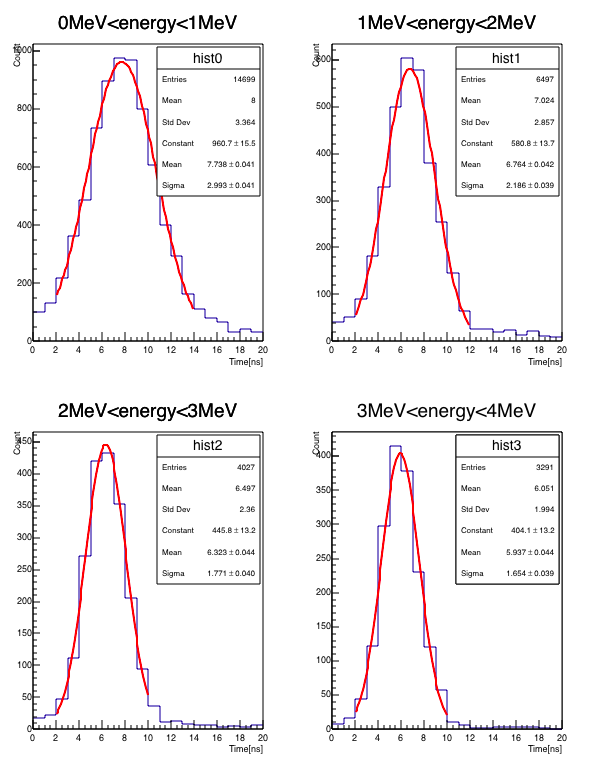
\includegraphics[width  = 0.8\textwidth]{figure/mino/gausfitting_ratio.eps}
\caption{0-4~MeVの低エネルギーのイベントを1~MeV 毎に区切って時刻をガウシアンでフィッティング}
\label{fig:NaI_peak_gaus_fitting}
\end{minipage}
\begin{minipage}{0.5\hsize}
\centering
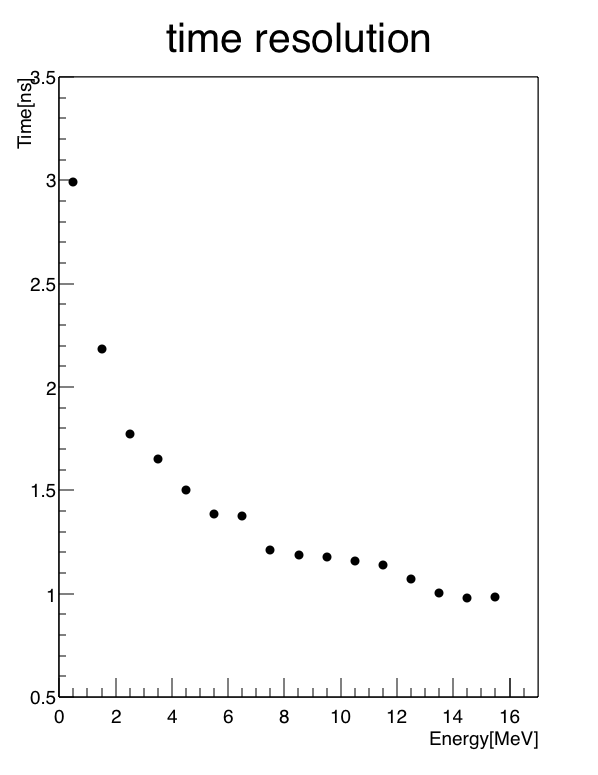
\includegraphics[width  = 0.8\textwidth]{figure/mino/timeresolution_ratio.eps}
\caption{1~MeV 毎に時間分解能をプロット}
\label{fig:NaI_peak_time_resolution}
\end{minipage}
\end{figure}

%-------- lifetime fitting ----------------------------------------------------------

\subsubsection{ミューオン寿命解析}
銅板標的を用いたRUN15 のデータからミューオンの寿命を求めた.
得られた時間分布に対して以下の式~\eqref{eq:lifetime} で表される関数$f(t)$を用いてフィッティングを行った.バックグラウンドの影響を加味して定数項を加えた.
RUN15 のデータは4120~ns までしかデータを記録していなかったため,フィッティング範囲は1200~ns から4000~ns とした.
誤差はフィッティング時の統計によるものである.
%プラスチックシンチレータ側は定数項を含まないフィッティングもしている。
\begin{gather}
f(t) = A\exp(-t / \tau)+C \label{eq:lifetime}
\end{gather}
結果は $\tau = 2.184 \pm 0.052~\mu \mathrm{s}$~となった.
\begin{figure}[H]
\centering
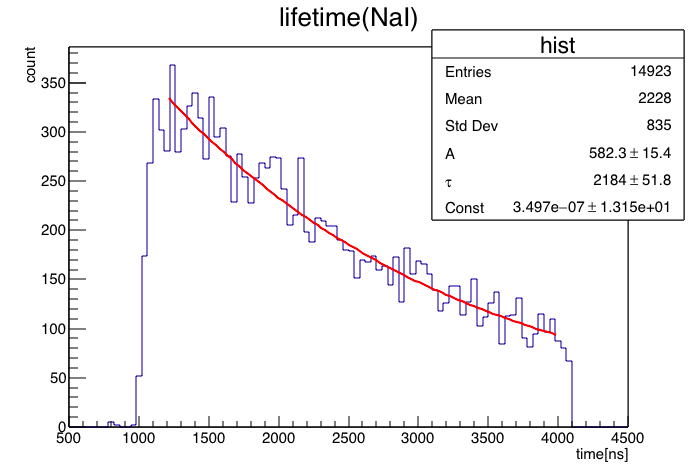
\includegraphics[width  = 0.7\textwidth]{figure/mino/lifetime_NaI_ratio.eps}
\caption{寿命フィッティング}
\end{figure}

%--------- g factor ---------------------------------------------------------------

\subsubsection{ミューオン$g$ 因子解析}

次に磁場標的を用いたRUN18 とRUN19 の解析からミューオンの$g$ 因子を求めた.RUN18 のデータは全event を用いて解析を行ったが,RUN19 は先述の通り途中で磁石が外れて磁場の値が変化したため,磁場の変化を確認した結果から最初の30000~events を除いたデータを用いた.

RUN18 とRUN19 から得られた時間分布に対して式\eqref{eq:gfactor} で表される関数$g(t)$を用いてフィッティングを行った.ここで寿命解析の時と同様に定数項を加え,フィッティング範囲は振動がきちんと見えている1600~ns から8000~ns までとした.

RUN18 とRUN19 のフィッティング結果を表~\ref{tab:gfactor_result} にまとめる.
ただし表~\ref{tab:gfactor_result} における$g$ 因子の計算には,プラスチックシンチレータの場合と同様に各点の磁場をビームプロファイルのガウシアンで加重平均した値,RUN18では$B$=56.06~G,RUN19では$B$=53.97~G を用いた.
また,誤差はフィッティング時の統計により得られたものを載せており,磁場の影響を含めたものについては後述する.

\begin{gather}
g(t) = A\exp(-t / \tau)\{1+B\cos(\omega t+\delta)\}+C\label{eq:gfactor}
\end{gather}
\begin{table}[H]
\caption{フィッティングで得られたRUN18 とRUN19 の$\omega$ と$g$ 因子}
\centering
\begin{tabular}{cccc}\toprule
{} & $\tau~[\mu \mathrm{s}]$ & $\omega~[/\mu \mathrm{s}]$ & $g$ \\ \midrule
RUN18 & 2.010 $\pm$ 0.048 & 4.923 $\pm$ 0.024 & 2.086 $\pm$ 0.010  \\
RUN19 & 2.126 $\pm$ 0.030 & 4.630 $\pm$ 0.015 & 2.038 $\pm$ 0.007 \\ \bottomrule
\end{tabular}
\label{tab:gfactor_result}
\end{table}

\begin{figure}[H]
\begin{minipage}{0.5\hsize}
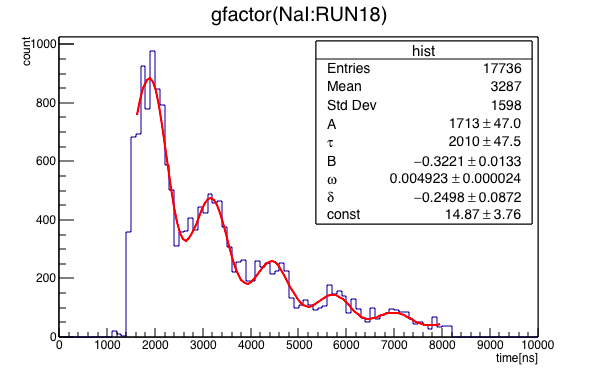
\includegraphics[width  = 1.0\textwidth]{figure/mino/gfactor_ratio_RUN18.eps}
\caption{RUN18 を用いた$g$ 因子のフィッティング}
\end{minipage}
\begin{minipage}{0.5\hsize}
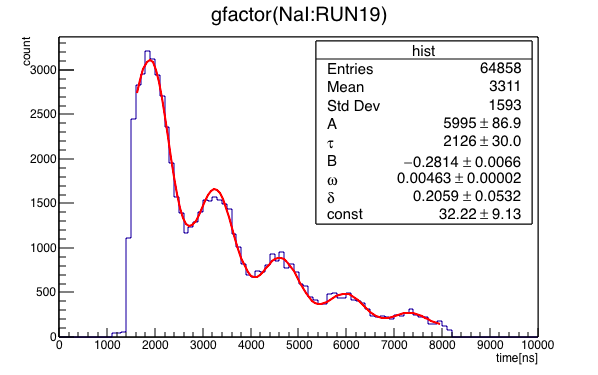
\includegraphics[width  = 1.0\textwidth]{figure/mino/gfactor_ratio_RUN19.eps}
\caption{RUN19 を用いた$g$ 因子のフィッティング}
\end{minipage}
\end{figure}

%-------- systematic error -------------------------------------------------------

\subsubsection{磁場の系統誤差について}

プラスチックシンチレータの場合と同様に,RUN18 とRUN19 の$g$ 因子解析に用いた磁場の値はビームプロファイルをもとに加重平均をとった値であるため,ビームの不定性による磁場の
加重平均の誤差を考察した.\\
ビーム強度のガウシアンの広がり$\sigma_{x},\sigma_{y}$ を動かしてRUN18 とRUN19 の場合での加重平均磁場の最大値と最小値を求めたところ表~\ref{tab:mag_max_min} のようになった.

\begin{table}[H]
\caption{$\sigma_{x},\sigma_{y}~[\mathrm{cm}]$ を動かした時の最大磁場と最小磁場}
\centering
\begin{tabular}{ccc}\toprule%最大磁場と最低磁場
{} & $B_\mathrm{max}~[\mathrm{G}]$ &  $B_\mathrm{min}~[\mathrm{G}]$   \\ \midrule
RUN18 & 56.58\;($\sigma_{x}=3.3,\sigma_{y}=1.0$) & 55.82\;($\sigma_{x}=3.9,\sigma_{y}=2.9$)  \\
RUN19 & 54.44\;($\sigma_{x}=3.9,\sigma_{y}=1.0$) & 53.76\;($\sigma_{x}=3.9,\sigma_{y}=1.0$) \\ \bottomrule
\end{tabular}
\label{tab:mag_max_min}
\end{table}

磁場が最大・最小,そしてもとのビームプロファイルのときの$g$ 因子を表\ref{tab:mag_g}に示す.また,磁場の測定誤差を含んだ$g$ 因子の統計誤差については,磁場の誤差$\delta B$ を考慮するとプラスチックシンチレータで求めた誤差伝播の式\eqref{eq:PSgosa}より,$g$ 因子の誤差$\sigma_{B}$ は表~\ref{tab:g_error} の値が得られた.

\begin{table}[H]
\caption{磁場$B$ の値とそれらに対応する$g$ 因子の値}
\centering
\begin{tabular}{cccc}\toprule%最大磁場と最低磁場
{} & $B_\mathrm{max}$ & $B$ & $B_\mathrm{min}$  \\ \midrule
RUN18 & 2.066 & 2.086 & 2.095 \\
RUN19 & 2.020 & 2.038 & 2.046 \\ \bottomrule
\end{tabular}
\label{tab:mag_g}
\end{table}

\begin{table}[H]%g因子の系統誤差(磁場)
\caption{磁場による$g$ 因子の誤差の伝播}
\centering
\begin{tabular}{ccc}\toprule
{} & $\delta B~[\mathrm{G}]$ &  $\sigma_{B}$  \\ \midrule
RUN18 & 1.20 & 0.046  \\
RUN19 & 2.36 & 0.089 \\ \bottomrule
\end{tabular}
\label{tab:g_error}
\end{table}

RUN18 とRUN19 の$g$ 因子の統計誤差と系統誤差を表\ref{tab:NaIggosamatome}にまとめる.
ここで誤差の第一項は磁場の影響を含めた統計誤差であり,第二項はビームプロファイルの不定性による系統誤差である.

\begin{table}[H]%g因子の誤差のまとめ
\caption{$g$ 因子の誤差のまとめ}
\centering
\begingroup
\renewcommand{\arraystretch}{1.2}%行間を変更
\begin{tabular}{cc}\toprule
{} &   $g$  \\ \midrule
RUN18 & $2.086 \pm 0.046^{+0.009}_{-0.020} $  \\
RUN19 & $2.038 \pm 0.089^{+0.008}_{-0.018} $  \\ \bottomrule
\end{tabular}\label{tab:NaIggosamatome}
\endgroup
\end{table}

二つの値をまとめて,$g = 2.062 \pm 0.050^{+0.009}_{-0.020}$ という値が得られた.ここで系統誤差は二つのうち大きい方を選んだ.

\subsubsection{プラスチックシンチレータとの位相差の確認}
\label{subsubsec:PhaseCheck}

NaI シンチレータとプラスチックシンチレータの$g$ 因子の解析から$\cos$ 振動の初期位相$\delta$ に注目すると,これら二つの位相差は実験中の物理的セットアップに起因していると考えられる.
実際,二つのシンチレータは標的に対しておよそ$87^{\circ}$ の角度をつけて配置していたため,それにともなって初期位相もおよそ$87^{\circ}$ 分の差をもっているはずである.

これらの事実を解析から確かめるために,まず二つの検出器から得られたデータの時間原点をそろえる必要がある.
これら二つの検出器間には時間分解能などの性能差もあるが,そもそも信号の伝送に用いたケーブルの長さが違うために時間原点がそろっていない.
今回は時間原点をそろえるために\ref{subsubsec:PSLife} でものべた高速$e^{+}$ 粒子による小さなピークを用いることを考えた.
今回のセットアップにおいて二つの検出器からビーム出口までの長さはビームライン全体の長さに比べると小さく,生成ターゲットから二つの検出器までに$e^{+}$ が飛来するまでの時間はほぼ等しいと考えられるので,このピークをそろえることで時間原点とすることができる.
NaI シンチレータの$e^{+}$ ピーク探索とそれを用いた原点調整後のヒストグラムを図~\ref{fig:NaITimeOrigin}に示す.また,プラスチックシンチレータで同様のことを行ったものを図~\ref{fig:PSTimeOrigin} に示す.
\begin{figure}[h]
	\centering
	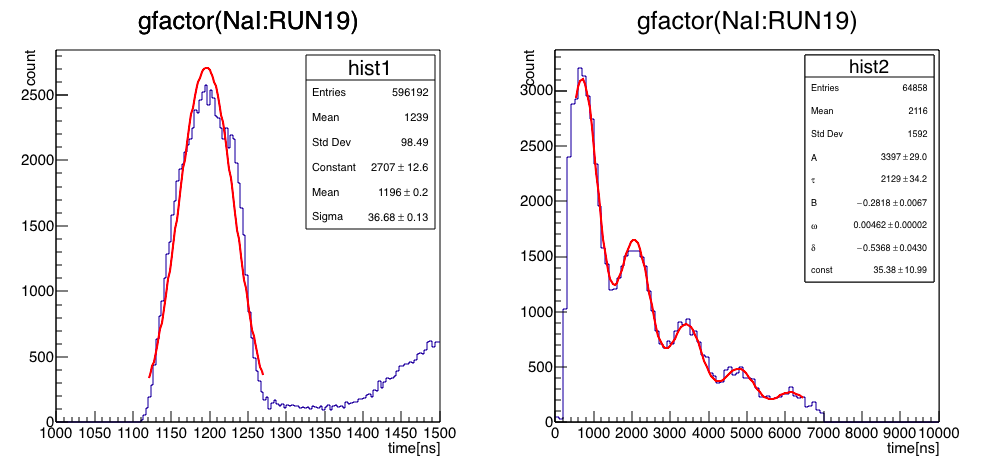
\includegraphics[width = 0.9\textwidth]{figure/mino/NaITimeOrigin.eps}
	\caption{(左) NaI シンチレータにおける$e^{+}$ イベントの時刻分布.(右) 原点調節後のヒストグラム}
	\label{fig:NaITimeOrigin}
	%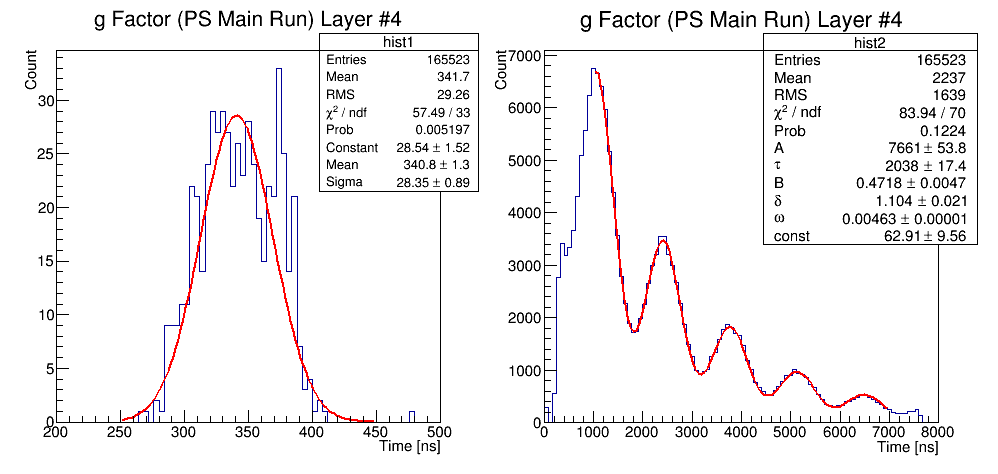
\includegraphics[width = 0.9\textwidth]{figure/mino/PSTimeOrigin.png}
	\includegraphics[width = 0.9\textwidth]{figure/mino/PSOriginCheck.eps}
	\caption{(左) プラスチックシンチレータにおける$e^{+}$ イベントの時刻分布.(右) 原点調節後のヒストグラム}
	\label{fig:PSTimeOrigin}
\end{figure}

それぞれのフィッティングから得られた初期位相$\delta$ を表\ref{tab:InitPhases} に示す.
\begin{table}[h]
	\centering
	\caption{各検出器の初期位相}
	\begin{tabular}{cc}\toprule
	検出器 & $\delta~[\mathrm{rad.}]$ \\ \midrule
	NaI シンチレータ & $-0.54 \pm 0.04$ \\
	プラスチックシンチレータ & $\phantom{-}1.11 \pm 0.02$ \\ \bottomrule
	\end{tabular}\label{tab:InitPhases}
\end{table}%
表\ref{tab:InitPhases} から位相差は$1.65 \pm 0.06 \sim \pi / 2$ となり,セットアップの角度と整合していることが確認できた.

%\end{document}
